\documentclass{article}
\usepackage{fullpage}
\usepackage{indentfirst}
\usepackage{amsmath}
\usepackage{amsfonts}
\usepackage{array}
\usepackage{tipa}
\usepackage{tikz}
\usepackage{tikz-qtree}
\usetikzlibrary{matrix, arrows, automata}
\usepackage{natbib}
\usepackage{gb4e}
\noautomath
\newcommand{\Y}{$\checkmark$}
\newcommand{\R}{$\Rightarrow$}
\newcommand\myeq{\mathrel{\stackrel{\makebox[0pt]{\mbox{\normalfont\tiny def}}}{=}}}
\newcommand{\ap}{\approx}
\title{Terminal Spread in Gao'an}
\author{Chris Oakden}
\begin{document}
\maketitle
Consider the following data from Gao'an \citep{Bao1990, Yan1981}:
\begin{center}
\begin{tabular}[t]{lll}
\textipa{CiEu} & han & `make charcoal' \\
55 & 33 & base form \\
53 & 33 & sandhi form\\
\hspace{1em} \\
\textipa{soN} & \textipa{tCi} & `bi-seasonal' \\
55 & 33 & base form \\
53 & 33 & sandhi form\\
\end{tabular}
\hspace{1cm}
\begin{tabular}[t]{lll}
\textipa{kuN} & \textipa{Cia} & `commune' \\
55 & 11 & base form \\
53 & 11 & sandhi form\\
\hspace{1em} \\
\textipa{ka} & \textipa{p\super hEi} & `double' \\
55 & 11 & base form \\
53 & 11 & sandhi form\\
\end{tabular}
\end{center}
Bao interprets these data as evidence of local spreading of \emph{terminal tonal nodes}; [l] tone (either [L] as -u;l or [M] as +u;l) spreads regressively to a heterosyllabic high-registered [H] tone. This is represented graphically for /H.M/$\mapsto$[HM.M], again assuming tier conflation.
\begin{center}
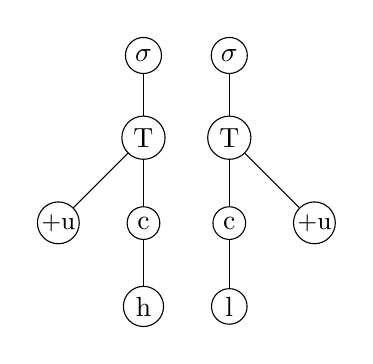
\begin{tikzpicture} [baseline = (y1.base)]
\matrix (m) [matrix of nodes, column sep = 1.5em, row sep = 1.5em]{
& \node[draw,circle, inner sep =2pt](x1){$\sigma$};  &  \node[draw,circle, inner sep =2pt](x2){$\sigma$};  \\
& \node[draw,circle, inner sep =2pt](y1){T}; &   \node[draw,circle, inner sep =2pt](y2){T}; \\
\node[draw,circle, inner sep =.5pt](z1){\small +u}; & \node[draw,circle, inner sep =2pt](z2){c}; &   \node[draw,circle, inner sep =2pt](z3){c}; & \node[draw,circle, inner sep =.5pt](z4){\small +u}; \\
 & \node[draw,circle, inner sep =2pt](t2){h}; &  \node[draw,circle, inner sep =2pt](t3){l}; \\
};
\draw (x1) -- (y1);
\draw (x2) -- (y2);
\draw (z1) -- (y1);
\draw (z2) -- (y1);
\draw (z2) -- (t2);
\draw (y2) -- (z3);
\draw (y2) -- (z4);
\draw (z3) -- (t3);
\end{tikzpicture}
\hspace{.3cm}
$\rightarrow$
\hspace{.3cm}
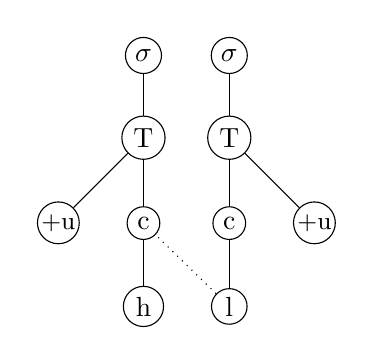
\begin{tikzpicture} [baseline = (y1.base)]
\matrix (m) [matrix of nodes, column sep = 1.5em, row sep = 1.5em]{
& \node[draw,circle, inner sep =2pt](x1){$\sigma$};  &  \node[draw,circle, inner sep =2pt](x2){$\sigma$};  \\
& \node[draw,circle, inner sep =2pt](y1){T}; &   \node[draw,circle, inner sep =2pt](y2){T}; \\
\node[draw,circle, inner sep =.5pt](z1){\small +u}; & \node[draw,circle, inner sep =2pt](z2){c}; &   \node[draw,circle, inner sep =2pt](z3){c}; & \node[draw,circle, inner sep =.5pt](z4){\small +u}; \\
 & \node[draw,circle, inner sep =2pt](t2){h}; &  \node[draw,circle, inner sep =2pt](t3){l}; \\
};
\draw (x1) -- (y1);
\draw (x2) -- (y2);
\draw (z1) -- (y1);
\draw (z2) -- (y1);
\draw (z2) -- (t2);
\draw (y2) -- (z3);
\draw (y2) -- (z4);
\draw (z3) -- (t3);
\draw [dotted] (t3) -- (z2);
\end{tikzpicture}
\hspace{.3cm}
$\rightarrow$
\hspace{.3cm}
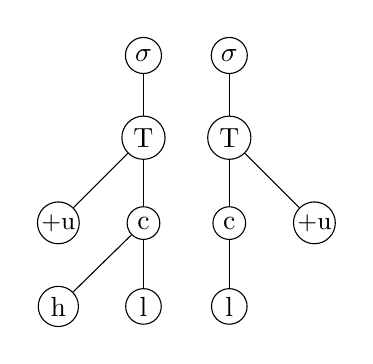
\begin{tikzpicture} [baseline = (y1.base)]
\matrix (m) [matrix of nodes, column sep = 1.5em, row sep = 1.5em]{
& \node[draw,circle, inner sep =2pt](x1){$\sigma$};  &  \node[draw,circle, inner sep =2pt](x2){$\sigma$};  \\
& \node[draw,circle, inner sep =2pt](y1){T}; &   \node[draw,circle, inner sep =2pt](y2){T}; \\
\node[draw,circle, inner sep =.5pt](z1){\small +u}; & \node[draw,circle, inner sep =2pt](z2){c}; &   \node[draw,circle, inner sep =2pt](z3){c}; & \node[draw,circle, inner sep =.5pt](z4){\small +u}; \\
  \node[draw,circle, inner sep =2pt](t1){h};& \node[draw,circle, inner sep =2pt](t2){l}; &  \node[draw,circle, inner sep =2pt](t3){l}; \\
};
\draw (x1) -- (y1);
\draw (x2) -- (y2);
\draw (z1) -- (y1);
\draw (z2) -- (y1);
\draw (z2) -- (t2);
\draw (y2) -- (z3);
\draw (y2) -- (z4);
\draw (z3) -- (t3);
\draw (t1) -- (z2);
\end{tikzpicture}
\end{center}
Crucially, this sandhi pattern only applies to level low/mid tones spreading regressively to high level tones. Contour tones do not participate in the alternation, nor does the data exhibit any evidence of high-tone spread. \par
We may formalize this spread as a logical transduction in a similar fashion as spreading on higher tiers, that is, by generating a copy of the spreading tone in a separate copy set, and defining domination such that the tone \emph{spreads} regressively to an adjacent syllable. Syllable, `T' root, and contour `c' nodes do not change from input to output, so their unary relation definitions are omitted. Register features do not change as a result of sandhi, but their definition is relevant as only specific combinations trigger the alternation. Unary relations defined over the second copy set other than the [l] terminal are set to $\mathtt{False}$.  
\begin{equation}
\begin{aligned}
P^{1}_{+u}(x)&\myeq P_{r}(x) & P^{1}_{-u}(x)&\myeq P_{r}(x)\land \neg pnlt(x) \\
P^{1}_{l}(x)&\myeq P_{l}(x)\land final(x) & P^{1}_{h}(x)&\myeq P_{h}(x)\land pnlt(\delta(x))\land \neg(pnlt(\delta(succ(x)))) \\
P^{1}_{l}(x)&\myeq P_{l}(x)\land final(x) \\
\end{aligned}
\end{equation}
These unary relation definitions ensure that regressive terminal-l spreading are predicted only in observed contexts. Sequences of two [+u]-registered syllables or a [+u.-u] sequence will trigger spreading, but no others (via the definitions of $P^{1}_{+u}(x)$ and $P^{1}_{-u}(x)$). Definitions of tonal elements achieve the same result; only a high level tone followed by either a mid (+u;l) or low (-u;l) level tone will trigger sandhi. As before, the spreading element is generated in the second copy set, in this case a single terminal node.\par
Association does not change, so it is omitted here. Note that association between copy sets and within the second copy set are set to $\mathtt{False}$ The dominance functions are as below:
\begin{equation}
\begin{aligned}
\delta^{1,1}(x)\ap y&\myeq \delta(x)\ap y & \delta^{1,2}(x)\ap y&\myeq \mathtt{False} \\
\delta^{2,1}(x)\ap y&\myeq P_{l}(x)\land P_{c}(y)\land final(x)\land pnlt(y) & \delta^{2,2}(x)\ap y&\myeq \mathtt{False} \\
\end{aligned}
\end{equation}
Between the input and the first copy set of the output, no changes are observed in domination relations, so it is defined identical to the input. Domination from the second copy set to the first achieves regressive spread. \par
Linear order of structural nodes does not change between input and output with the exception of the terminal node tier, and in this case the change is rather complex. The successor of the initial [h] node in the first copy set is the [l] node in the second copy set, and its successor is its equivalent in the first copy set (which itself is the final element). To achieve this ordering, we define linear order over these nodes via $succ(x)\ap y$ thus:
\begin{equation}
\begin{aligned}
succ^{1,1}(x)\ap y&\myeq P_{l}(x)\land P_{l}(y)\land x \ap y \\
succ^{1,2}(x)\ap y&\myeq P_{h}(x)\land P_{l}(y) \land pnlt(\delta(x)) \land \neg(pnlt(\delta(succ(x))))\land final(y) \\
succ^{2,1}(x)\ap y&\myeq P_{l}(x) \land P_{l}(y)\land x \ap y \\
succ^{2,2}(x)\ap y&\myeq \mathtt{False} \\
\end{aligned}
\end{equation}
Applying this transduction to a model of a /H.M/ sequence (+u;h followed by +u;l) yields:
\begin{center}
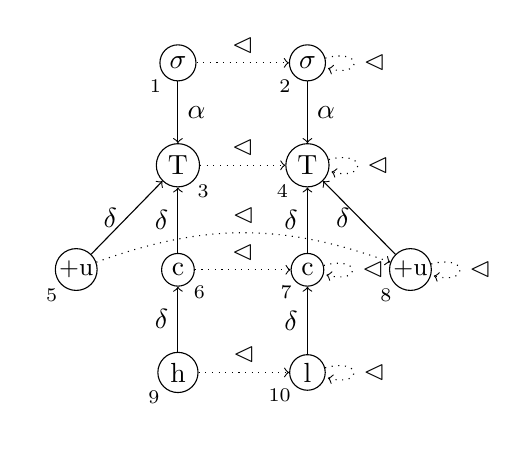
\begin{tikzpicture} [baseline = (y1.base)]
\matrix (m) [matrix of nodes, column sep = 1.5em, row sep = 1.5em]{
& \node[draw,circle, inner sep =2pt, label ={[label distance = -3pt] below left:\scriptsize1}](x1){$\sigma$};  &  \node[draw,circle, inner sep =2pt, label ={[label distance = -3pt] below left:\scriptsize2}](x2){$\sigma$};  \\
& \node[draw,circle, inner sep =2pt, label ={[label distance = -3pt] below right:\scriptsize3}](y1){T}; &   \node[draw,circle, inner sep =2pt, label ={[label distance = -3pt] below left:\scriptsize4}](y2){T}; \\
\node[draw,circle, inner sep =.5pt, label ={[label distance = -3pt] below left:\scriptsize5}](z1){\small +u}; & \node[draw,circle, inner sep =2pt, label ={[label distance = -3pt] below right:\scriptsize6}](z2){c}; &   \node[draw,circle, inner sep =2pt, label ={[label distance = -3pt] below left:\scriptsize7}](z3){c}; & \node[draw,circle, inner sep =.5pt, label ={[label distance = -3pt] below left:\scriptsize8}](z4){\small +u}; \\
& \node[draw,circle, inner sep =2pt, label ={[label distance = -3pt] below left:\scriptsize9}](t2){h}; &  \node[draw,circle, inner sep =2pt, label ={[label distance = -3pt] below left:\scriptsize10}](t3){l}; &  \\
};
\draw [->] (x1) -- (y1) node[right, pos=.5]{$\alpha$};
\draw [->] (x2) -- (y2) node[right, pos=.5]{$\alpha$};
\draw [->] (z1) -- (y1) node[left, pos=.5]{$\delta$};
\draw [->] (z2) -- (y1) node[left, pos=.5]{$\delta$};
\draw [->] (z3) -- (y2) node[left, pos=.5]{$\delta$};
\draw [->] (z4) -- (y2) node[left, pos=.5]{$\delta$};
\draw [->] (t2) -- (z2) node[left, pos=.5]{$\delta$};
\draw [->] (t3) -- (z3) node[left, pos=.5]{$\delta$};
\draw [->, dotted] (x1) -- (x2) node[above,pos=.5]{$\vartriangleleft$};
\draw [->, dotted] (y1) -- (y2) node[above,pos=.5]{$\vartriangleleft$};
\draw [->, dotted] (z2) -- (z3) node[above,pos=.5]{$\vartriangleleft$};
\draw [->, dotted] (t2) -- (t3) node[above,pos=.5]{$\vartriangleleft$};
\path [->, dotted] (z1) edge[bend left=20] node[above,pos=.5]{$\vartriangleleft$} (z4);
\path [->, dotted] (x2) edge[loop right] node{$\vartriangleleft$} (x2);
\path [->, dotted] (y2) edge[loop right] node{$\vartriangleleft$} (y2);
\path [->, dotted] (z3) edge[loop right] node{$\vartriangleleft$} (z3);
\path [->, dotted] (z4) edge[loop right] node{$\vartriangleleft$} (z4);
\path [->, dotted] (t3) edge[loop right] node{$\vartriangleleft$} (t3);
\end{tikzpicture}
\hspace{.5cm}
$\mapsto$
\hspace{.5cm}
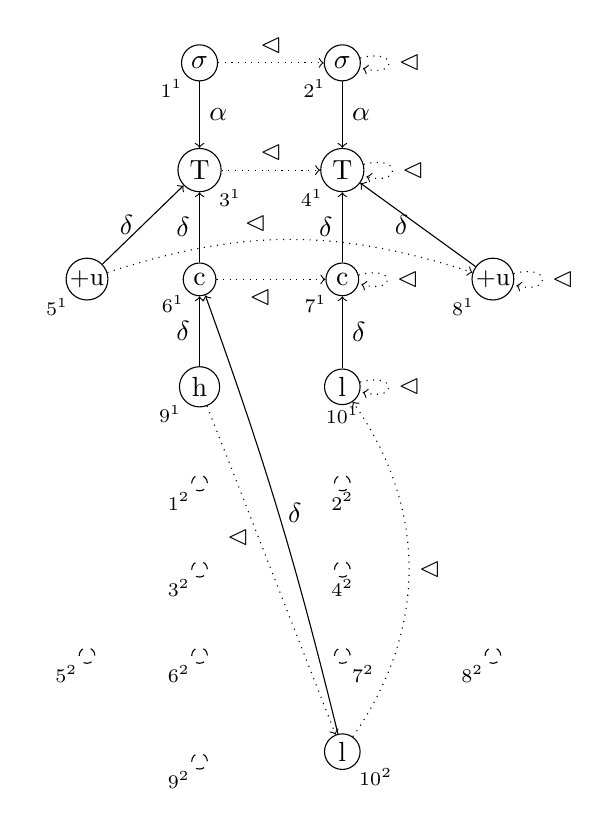
\begin{tikzpicture} [baseline = (y1.base)]
\matrix (m) [matrix of nodes, column sep = 1.5em, row sep = 1.5em]{
& \node[draw,circle, inner sep =2pt, label ={[label distance = -3pt] below left:\scriptsize$1^1$}](x1){$\sigma$};  &  \node[draw,circle, inner sep =2pt, label ={[label distance = -3pt] below left:\scriptsize$2^1$}](x2){$\sigma$};  \\
& \node[draw,circle, inner sep =2pt, label ={[label distance = -3pt] below right:\scriptsize$3^1$}](y1){T}; &   \node[draw,circle, inner sep =2pt, label ={[label distance = -3pt] below left:\scriptsize$4^1$}](y2){T}; \\
\node[draw,circle, inner sep =.5pt, label ={[label distance = -3pt] below left:\scriptsize$5^1$}](z1){\small +u}; & \node[draw,circle, inner sep =2pt, label ={[label distance = -3pt] below left:\scriptsize$6^1$}](z2){c}; &   \node[draw,circle, inner sep =2pt, label ={[label distance = -3pt] below left:\scriptsize$7^1$}](z3){c}; & \node[draw,circle, inner sep =.5pt, label ={[label distance = -3pt] below left:\scriptsize$8^1$}](z4){\small +u}; \\
& \node[draw,circle, inner sep =2pt, label ={[label distance = -3pt] below left:\scriptsize$9^1$}](t2){h}; &  \node[draw,circle, inner sep =2pt, label ={[label distance = -3pt] below:\scriptsize$10^1$}](t3){l}; &  \\
& \node[draw,circle, dashed, inner sep =2pt, label ={[label distance = -3pt] below left:\scriptsize$1^2$}]{\hspace{1em}}; & \node[draw,circle, dashed, inner sep =2pt, label ={[label distance = -3pt] below:\scriptsize$2^2$}]{\hspace{1em}}; \\
& \node[draw,circle, dashed, inner sep =2pt, label ={[label distance = -3pt] below left:\scriptsize$3^2$}]{\hspace{1em}}; & \node[draw,circle, dashed, inner sep =2pt, label ={[label distance = -3pt] below:\scriptsize$4^2$}]{\hspace{1em}}; \\
\node[draw,circle, dashed, inner sep =2pt, label ={[label distance = -3pt] below left:\scriptsize$5^2$}]{\hspace{1em}}; & \node[draw,circle, dashed, inner sep =2pt, label ={[label distance = -3pt] below left:\scriptsize$6^2$}]{\hspace{1em}}; & \node[draw,circle, dashed, inner sep =2pt, label ={[label distance = -3pt] below right:\scriptsize$7^2$}](z22){\hspace{1em}};  & \node[draw,circle, dashed, inner sep =2pt, label ={[label distance = -3pt] below left:\scriptsize$8^2$}]{\hspace{1em}}; \\
& \node[draw,circle, dashed, inner sep =2pt, label ={[label distance = -3pt] below left:\scriptsize$9^2$}]{\hspace{1em}}; & \node[draw,circle, inner sep =2pt, label ={[label distance = -3pt] below right:\scriptsize$10^2$}](t22){l}; \\ 
};
\draw [->] (x1) -- (y1) node[right, pos=.5]{$\alpha$};
\draw [->] (x2) -- (y2) node[right, pos=.5]{$\alpha$};
\draw [->] (z1) -- (y1) node[left, pos=.5]{$\delta$};
\draw [->] (z3) -- (y2) node[left, pos=.5]{$\delta$};
\draw [->] (z4) -- (y2) node[left, pos=.5]{$\delta$};
\draw [->] (t3) -- (z3) node[right, pos=.5]{$\delta$};
\draw [->] (t2) -- (z2) node[left, pos=.5]{$\delta$};
\draw [->] (z2) -- (y1) node[left, pos=.5]{$\delta$};
\path [->] (t22) edge[bend right=3] node[right, pos=.5]{$\delta$} (z2);
\draw [->, dotted] (x1) -- (x2) node[above,pos=.5]{$\vartriangleleft$};
\draw [->, dotted] (y1) -- (y2) node[above,pos=.5]{$\vartriangleleft$};
\draw [->, dotted] (z2) -- (z3) node[below,pos=.4]{$\vartriangleleft$};
\draw [->, dotted] (t2) -- (t22) node[left,pos=.4]{$\vartriangleleft$};
\path [->, dotted] (z1) edge[bend left=18] node[above,pos=.4]{$\vartriangleleft$} (z4);
\path [->, dotted] (t22) edge [bend right=35]node[right,pos=.5]{$\vartriangleleft$} (t3);
\path [->, dotted] (x2) edge[loop right] node{$\vartriangleleft$} (x2);
\path [->, dotted] (y2) edge[loop right] node{$\vartriangleleft$} (y2);
\path [->, dotted] (z3) edge[loop right] node{$\vartriangleleft$} (z3);
\path [->, dotted] (z4) edge[loop right] node{$\vartriangleleft$} (z4);
\path [->, dotted] (t3) edge[loop right] node{$\vartriangleleft$} (t3);
\end{tikzpicture}
\end{center}
\bibliographystyle{apalike}
\bibliography{references}
\end{document}